\chapter{Problem solving}

\setcounter{problem}{1}

\section{Some questions to get you warmed up}


{\bf Q}. You intercept an encrypted message from another student and you would like to decrypt it because you are nosy. Let's assume that the student mapped each letter of the alphabet to a different, unique letter chosen at random. How would you go about decrypting this message? Is it even possible if the mapping is truly random?

\begin{marginfigure}[-1.2in]
\begin{center}
\scalebox{.8}{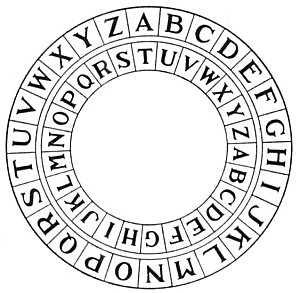
\includegraphics{figures/cipher.jpg}}
\end{center}
\caption{\tiny From {\tt http://www.sacred-texts.com/eso/sta/sta42.htm}}
\end{marginfigure}


\vspace{15mm}

\noindent {\bf Q}. Geophysicists like to explode dynamite and measure the direct and reflection waves using a ``pen on rolling paper'' device like a seismograph.  You find yourself in a remote location examining the signal from such a device and need to compute the area under the curve. The only tools you have with you are spare paper, pencil, sharp razor, ruler, and a sensitive scale. How can you get a reasonably accurate measure of the area under the seismograph curve in between two points?

\begin{marginfigure}[-1.8in]
\begin{center}
\scalebox{1}{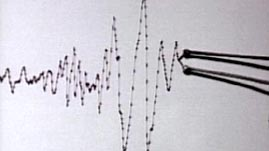
\includegraphics{figures/ess05_vid_seismograph_l.jpg}}
\end{center}
\caption{\tiny From  {\tt http://www.pbs.org/wgbh/nova/education/earth}}
\end{marginfigure}

\vspace{15mm}

\noindent {\bf Q}.  Imagine there is no symbolic solution to the area under the curve of $f(x) = \sin(x) + \frac{1}{3} \sin(3x)$ from $0$ to $\pi$. How could you estimate the area? Hint: do you like playing darts?

\begin{marginfigure}
\begin{center}
\scalebox{1}{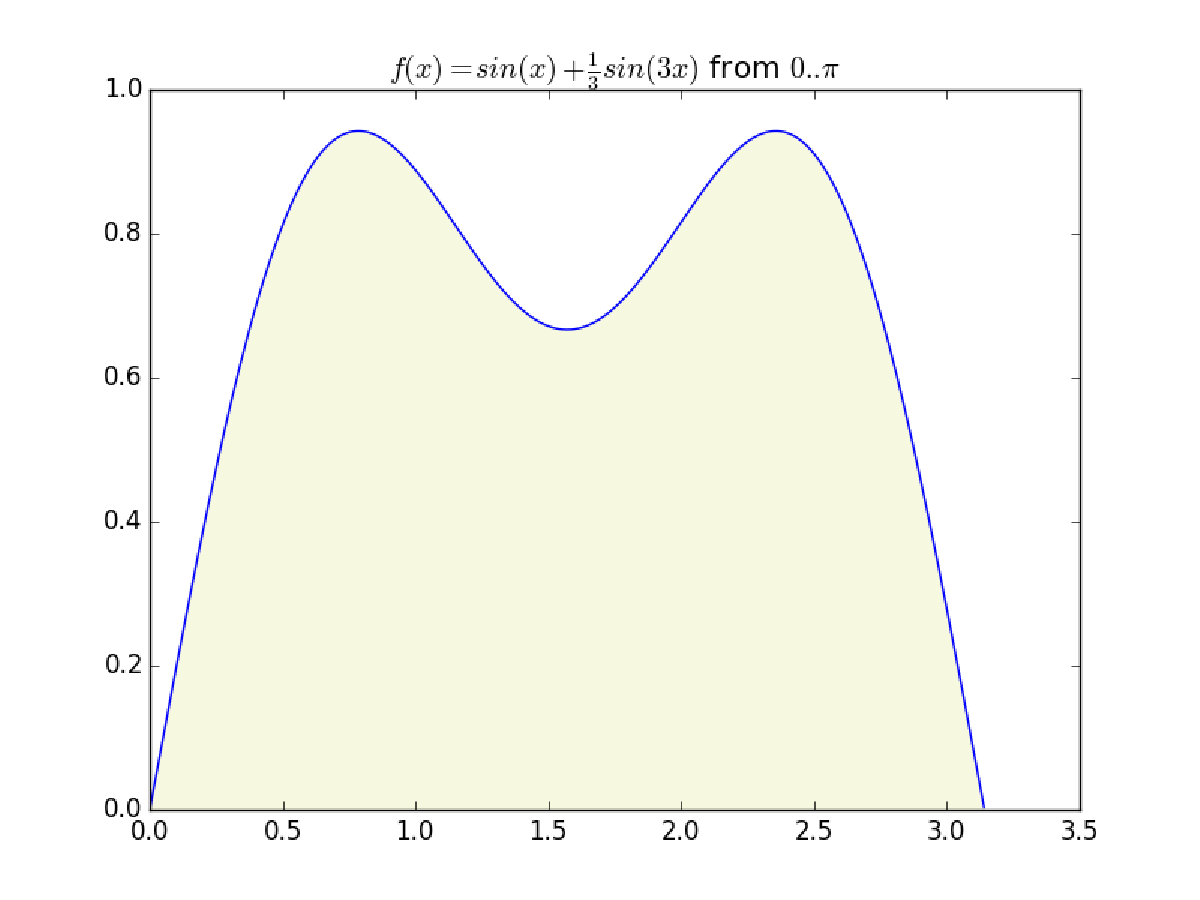
\includegraphics{figures/sin-curve.pdf}}
\end{center}
\end{marginfigure}

\vspace{20mm}

\noindent {\bf Q}.  How can you sort $N$ numbers in $[0,M]$ if you can only look at each number once?

\begin{marginfigure}
\begin{center}
\scalebox{1}{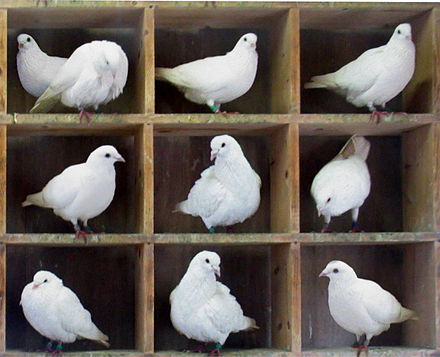
\includegraphics{figures/pigeons.jpg}}
\end{center}
\caption{\tiny From  {\tt https://en.wikipedia.org/wiki/Pigeonholing}}
\end{marginfigure}